\documentclass[12pt, a4paper,titlepage]{article}
\usepackage[italian]{babel}
\usepackage[utf8]{inputenc}
\usepackage{graphicx}
\usepackage[tc]{titlepic}
\usepackage{eurosym}
\usepackage{epstopdf}
\usepackage{pdflscape}
\usepackage[margin=2.5cm]{geometry}
\usepackage{float}
\usepackage{listings}
\usepackage[usenames,dvipsnames]{color}
\usepackage{hyperref}
\hypersetup{
    colorlinks=true,
    linkcolor=black
}
\usepackage{booktabs}
\graphicspath{{./pic/}}
\usepackage{fancyhdr}% http://ctan.org/pkg/fancyhdr
\usepackage{lastpage}
\usepackage{pifont}
\newcommand{\cmark}{\ding{51}}%
\newcommand{\xmark}{\ding{55}}%
\fancyhf{}% Clear header/footer
\fancyfoot[L]{\textsc{Piano di lavoro}}
\fancyfoot[R]{\thepage\ di \pageref{LastPage}}% \fancyfoot[R]{\thepage}
\renewcommand{\headrulewidth}{0pt}% Default \headrulewidth is 0.4pt
\renewcommand{\footrulewidth}{0.4pt}% Default \footrulewidth is 0pt

%fine impostazioni
\begin{document}
\begin{titlepage}

\newcommand{\HRule}{\rule{\linewidth}{0.5mm}} % Defines a new command for the horizontal lines, change thickness here

\center % Center everything on the page

%----------------------------------------------------------------------------------------
% HEADING SECTIONS
%----------------------------------------------------------------------------------------

\vspace*{\fill}
\textsc{\Large Università degli Studi di Padova}\\[0.5cm] % Major heading such as course name
\textsc{\large Corso di Laurea Magistrale in Informatica}\\[0.5cm] % Minor heading such as course title

%----------------------------------------------------------------------------------------
% TITLE SECTION
%----------------------------------------------------------------------------------------

\HRule \\[0.4cm]
{ \huge \textbf{Web Information Management}\\[0.4cm] Analisi di usabilità di NintendoLife.com}\\[0.4cm] % Title of your document
\HRule \\[0.5cm]
\large{Anno Accademico 2016/2017}\\[1cm]

\includegraphics[scale=0.3]{logo}\\[1cm] % Include a department/university logo - this will require the graphicx package
%----------------------------------------------------------------------------------------
% AUTHOR SECTION
%----------------------------------------------------------------------------------------
Jacopo Cavallarin, 1131015
\vspace*{\fill}
% If you don't want a supervisor, uncomment the two lines below and remove the section above
%\Large \emph{Author:}\\
%John \textsc{Smith}\\[3cm] % Your name

%----------------------------------------------------------------------------------------
% LOGO SECTION
%----------------------------------------------------------------------------------------



%----------------------------------------------------------------------------------------

\vfill % Fill the rest of the page with whitespace

\end{titlepage}
\newpage
\tableofcontents
\listoffigures
\thispagestyle{empty}
\clearpage
\pagenumbering{arabic}
\pagestyle{fancy}

\section{Introduzione}
\label{sec:introduzione}
\subsection{Descrizione del sito in esame}
\begin{figure}[h]
\centering

\includegraphics[width=.5\textwidth]{Logo_sito}
\end{figure}
URL completa del sito: \url{http://www.nintendolife.com}\\
NintendoLife è un sito che raccoglie tutte le novità riguardanti i prodotti di Nintendo, la famosa azienda giapponese di videogiochi. Oltre a riportare le ultime notizie, il sito propone recensioni e anteprime (spesso accompagnate da video) dei principali titoli prodotti per le console Nintendo e dei titoli per smartphone prodotti da Nintendo.\\
Oltre agli articoli, il sito contiene un forum a cui gli utenti possono registrarsi per discutere su ogni cosa che riguarda il mondo Nintendo.
\subsection{Periodo di analisi}
L'analisi del sito è stata effettuata durante il mese di Maggio 2017.

\section{Analisi} % (fold)
\label{sec:analisi}
Di seguito viene esposta l'analisi di usabilità del sito. Per ogni sezione verrà fornita anche una lista di aspetti positivi \cmark e negativi \xmark (se presenti).

\emph{NB: le immagini riportate di seguito sono contenute nella cartella \texttt{pic}. È inoltre possibile cliccare le immagini per aprirle in una finestra separata.}
\subsection{Nome del sito}
\label{sec:nome-sito}
\begin{itemize}
    \item[\cmark] Il dominio è \texttt{.com}
    \item[\cmark] Non sono presenti trattini o altri caratteri simbolici
    \item[\cmark] È una semplice composizione di 2 parole (Nintendo, Life)
\end{itemize}
Il nome è nel complesso buono perché breve ed efficace: è facile intuire il contenuto del sito a partire dal nome.
\clearpage
\subsection{Homepage}
\label{sub:homepage}
Poiché la homepage del sito è molto lunga, la relativa immagine è stata spezzata in più parti. Per vedere l'immagine completa si consulti il file \href{pic/homepage_lunga.jpeg}{\underline{homepage\_lunga.jpeg}}.
\begin{figure}[h]
\centering
\href{pic/homepage1.png}{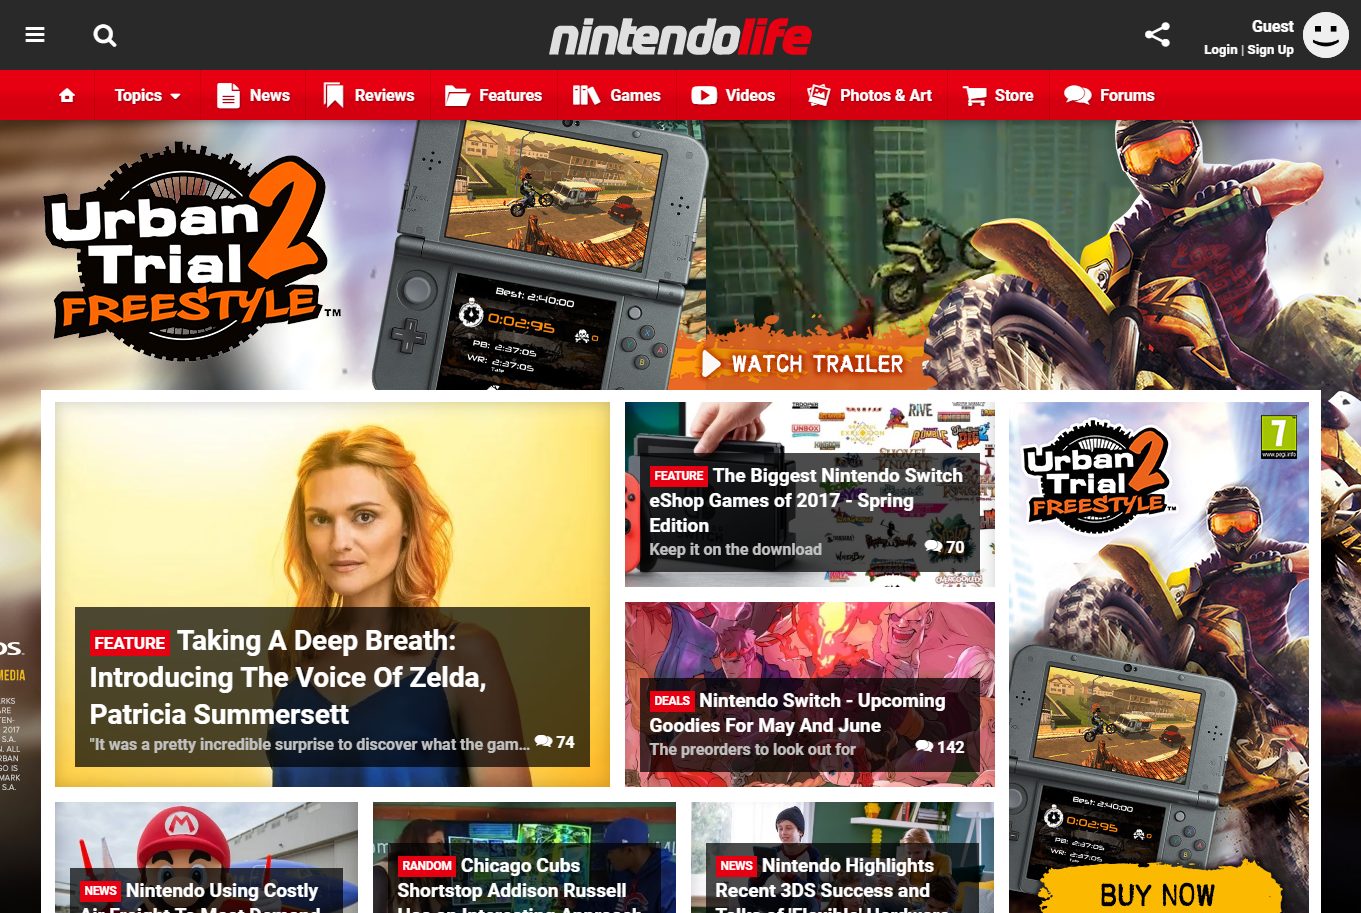
\includegraphics[width=.8\textwidth]{homepage1}}
\caption{\href{pic/homepage1.png}{Homepage del sito - prima schermata}}
\end{figure}

\section{Lista Immagini}
\label{sec:immagini}

\end{document}